\section{Introduction}

There are several studies supporting the central role of mechanical stimuli in tissue morphogenesis and homeostasis \cite{ex1,ex2}. In tissues, cells are mainly surrounded by extracellular matrix (ECM), a soft porous media made up of networks of polymer chains and charged proteins which is mixed with interstitial fluid. \textit{In vitro} studies have shown that ECM rigidity and shear stresses due to the flow of interstitial fluid can promote malignant phenotypes in a population of initially normal cells, impact on cell proliferation and differentiation \cite{ex3}. Further experiments have shown that tumour development is often associated with a stiffening of the tissue compared to the surrounding healthy one \cite{ex4}. This causes cells to be exposed to higher compressive stresses and the collapse of blood vessels, thus impeding the diffusion of substances in the extra-cellular environment. Hence, numerous therapies are less effective \cite{ecm2}. Based on such evidence, it is now widely accepted that, unlike originally thought, biological process are not simply regulated by biochemical signals but by the complex interplay of mechanical and chemical stimuli.
 
Given the different physical nature and scale of phenomena involved, coupling micro-environment and cell behaviours is a problem of high complexity. This requires understanding processes occurring at different temporal and spatial scales and how they interplay to determine the macroscopic behaviour of a tissue, whether healthy or damaged. Despite experiments probing the micro-scale are nowadays possible, these are usually limited to controlled environment in contrast to \textit{in vivo} conditions. On the other hand, macro-scale measurements are easier to gather, but give only information on average properties, which do not correspond to what cell experience. Hence, in order to manipulate the cell environment, we need quantitative models able to link this two scales. Having such knowledge, this could led to the development of novel therapies and completely change our approach to  drug design. In order for this to be possible, alongside experiments, it is necessary to develop a theoretical framework able to capture both the biology and physics involved and which is consistent with the known universal laws of Nature \cite{NET}. 

With the development of new experimental techniques such as Atomic Force Microscopy (AFM), the local mechanical properties of a material can be measured with nanometre precision \cite{viscoporo}. When tested at this scale, soft tissues and the ECM in particular have been found to be visco-elastic \cite{ex5}, independently from the presence of the interstitial fluid. Where purely elastic solids can only store energy when deformed, viscoelastic materials instead exhibit a time-dependent response to mechanical deformation as part of the energy is dissipated in the deformation process. This is associated with entropic favourable changes in the conformation of the ECM network itself. While a large amount of literature focuses on the poro-elastic properties of ECM, it remains unclear the role of viscosity in determining cell behaviour. However, the recent efforts to develop synthetic ECM, i.e. hydrogels, with tunable viscoelasticity, have now opened new research opportunities \cite{viscocell}. 

As discussed in Section \ref{ECMcomp}, from our point of view the ECM behaves as a polyelectrolyte gel \cite{ecm1,ecm2}, i.e. hydrogels with charged group. Besides being largely present in the natural world, synthetic polyelectrolytes are currently employed for a wide range of applications, such as drug delivery, biomedical devices, scaffolds for tissue engineering and soft robotics \cite{hydroex3,hydroex2,hydroex1,hydroex4}. Hence, there has been a growing interest in the soft matter community in understanding their behaviour and translating it into mathematical models. In particular, research has been focusing on the phenomena of swelling, i.e. large deformation due to absorption of water, and the diffusion transport and release of solution \cite{DROZDOV+,DROZDOVph,Reviewpolyel,swell2}. However, theoretical studies of viscoelastic soft materials remain limited. Most of the literature has been proposing poro-elastic models, which account for the dissipation of energy due to the transport of solutions but neglect the visco-elastic response of the material itself \cite{Article1}. While this assumption might be valid for certain applications, the empirical studies previously mentioned highlight the need of including this component in the study of living tissues.

As discussed in \cite{viscoporo}, there are spatial and time scales which allow to study the two independently. On one hand, nanoscale rheological testing with AFM give us information on the visco-elastic properties of the sample. For sufficiently small beads, the length scale considered in the experiment is so short that poroelastic relaxation is almost instantaneous and thus negligible. Different 1D rheological model are usually applied to fit experimental measurement: the most common for tissue and hydrogels is the \textit{Standard Linear Solid} model, see Figure \ref{SLS}, to fit the experimental data \cite{Article1,viscoporo}. The poro-elastic behaviour can instead be characterized by standard creep-relaxation test on whole sample. In this case, Darcy's law is usually applied to estimate the hydraulic conductivity and thus characterise the transport of fluid in the material \cite{Netti,viscoporo}. Despite having a good understanding of the two phenomena independently, there has been little attention to investigating how to two couple.
\begin{figure}
	\begin{subfigure}{0.45\textwidth}
		\centering 
		\def\svgwidth{1.3\linewidth}
		\input{latex/images/SLStand.pdf_tex}
		\caption{}
	\end{subfigure}
	\begin{subfigure}{0.45\textwidth}
	\centering
	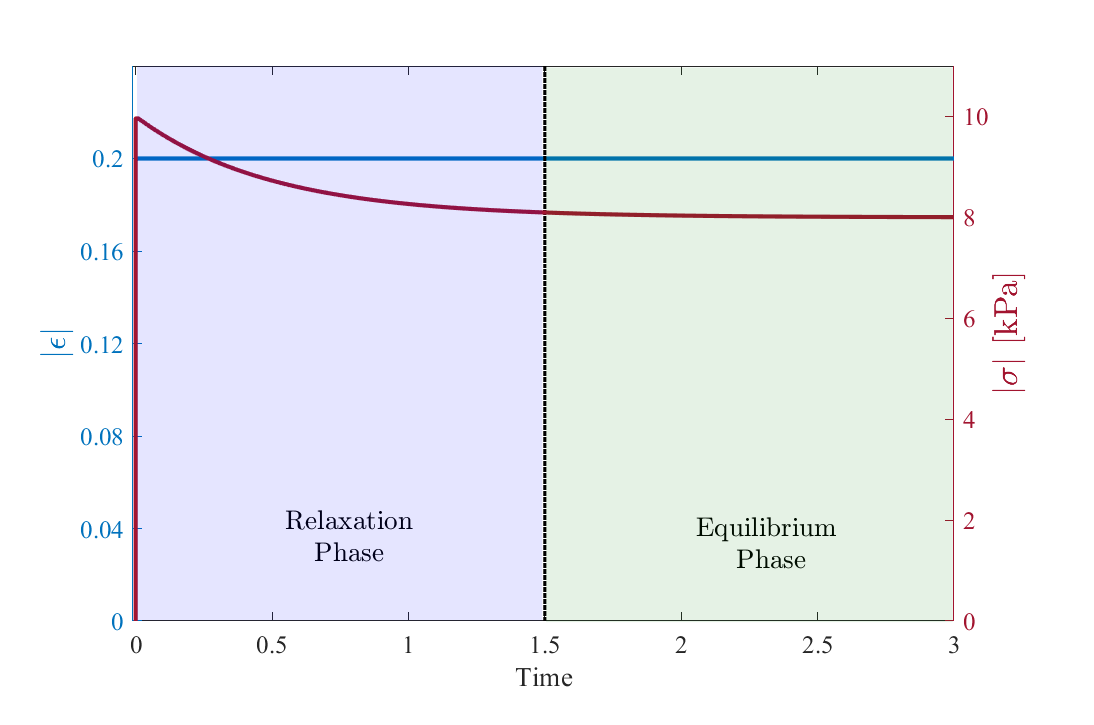
\includegraphics[scale=0.28]{images/SLS}\qquad 
	\caption{}
	\end{subfigure}

\vspace{5mm}
\begin{equation}
\begin{cases}
\sigma = (E_e+E_1)\epsilon-E_1\epsilon_d\\
\dot{\epsilon}_d + \frac{E_1}{\nu} \epsilon_d = \frac{E_1}{\nu} \epsilon
\end{cases}
\tag{SLS}
\end{equation}
\vspace{3mm}
\caption{1D Standard Linear Solid. (a) Rheological Model; (b) Standard Response to a compression test. (1) Differential Equation for the Standard Linear Solid model in the 1D case.}
\label{SLS}
\end{figure}

Our works aims to develop a continuum mathematical model of the extracellular matrix which is consistent with the laws of thermodynamics, which accounts for its poro-visco-elastic properties and the coupling of mechanical, transport and electrical phenomena. Nonetheless, our results are more widely applicable to the study of polyelectrolyte gels. At our present knowledge, there is no previous work in the literature capturing all these aspects in a thermodynamic consistent model. In \cite{ecm1,ecm2} Xue et al.~ develop a nonlinear poroelastic theory for ECM, which couples all three physical phenomena but does not include viscous dissipation. In \cite{Jeru}, the authors couple mechano-electrophysiological effects including the viscous dissipation but neglect transport; Caccavo et al.~ \cite{Article1} propose a poro-viscoelastic model for neutral hydrogel, thus excluding electrical effects.  Following these previous work, we will derive our model in the framework of linear non-equilibrium thermodynamics \cite{NET} accounting for multiple phases.


Despite the large number of studies that have characterised the poro-elastic and visco-elastic properties of ECM independently, little is known about their combined effect. In the literature, two main constitutive models have been presented, but never rigorously compared. Instead of arbitrarily choosing one of the two, we here develop both approaches, with the aim of identifying their differences and investigating experimental result which would allow us to experimentally test which one best describes the behaviour of soft tissues. 

Our work is organized as follows: in Section \ref{ECMcomp}, we discuss more in details the composition of the ECM. We then present a brief overview of Classical Irreversible Thermodynamics, which focuses on the principles later used in the derivation of our model in Section \ref{modeldev}. Common  [... FOLLOWING SECTIONS TO UPDATE AS I WRITE.]